\documentclass[12pt]{standalone}

\usepackage{tikz}
\usetikzlibrary{shapes,positioning,matrix}

\begin{document}
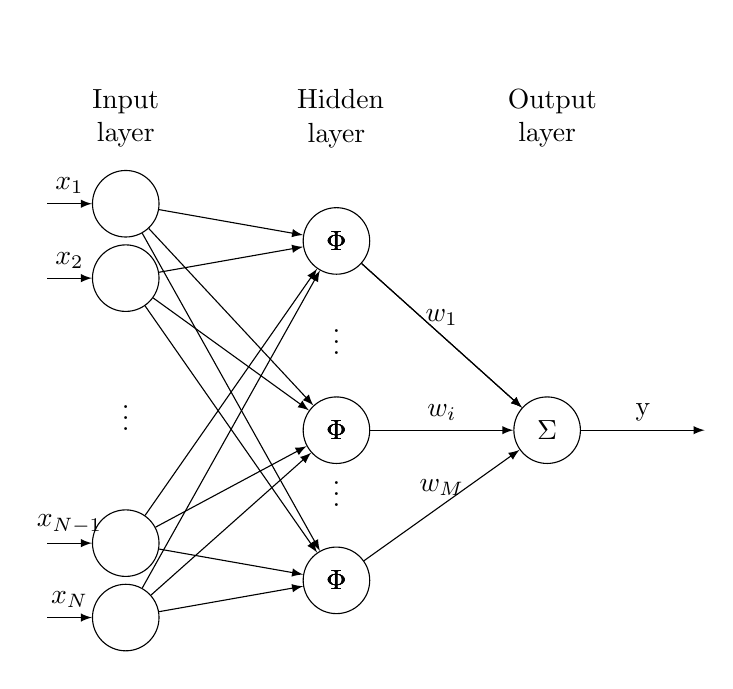
\begin{tikzpicture}[
plain/.style={
  draw=none,
  fill=none,
  },
net/.style={
  matrix of nodes,
  nodes={
    draw,
    circle,
    inner sep=8.5pt
    },
  nodes in empty cells,
  column sep=0.6cm,
  row sep=-11pt
  },
>=latex
]
\matrix[net] (mat)
{
|[plain]| \parbox{1cm}{\centering Input\\layer} & 
|[plain]| \parbox{1cm}{\centering Hidden\\layer} &
|[plain]| \parbox{1cm}{\centering Output\\layer} \\
& |[plain]| \\
|[plain]| & \\
& |[plain]| \\
|[plain]| & |[plain]| $\vdots$\\
|[plain]|$\vdots$& & \\
|[plain]| & |[plain]|$\vdots$ \\
& |[plain]| \\
|[plain]| & \\
& |[plain]| \\
};
\foreach \ai [count=\mi ]in {2,4}
     \draw[<-] (mat-\ai-1) -- node[above] {$x_\mi$} +(-1cm,0);
     \draw[<-] (mat-8-1) -- node[above] {$x_{N-1}$} +(-1cm,0);
     \draw[<-] (mat-10-1) -- node[above] {$x_{N}$} +(-1cm,0);
\foreach \ai in {2,4,8,10}
{\foreach \aii in {3,6,9}
  \draw[->] (mat-\ai-1) -- (mat-\aii-2)node(){$\Phi$};
}
  \draw[->] (mat-3-2) -- (mat-6-3)node(){$\Sigma$};
  \draw[->] (mat-3-2) --node[above]{$w_1$} (mat-6-3);
  \draw[->] (mat-6-2) --node[above]{$w_i$} (mat-6-3);
  \draw[->] (mat-9-2) --node[above]{$w_M$} (mat-6-3);
\draw[->] (mat-6-3) -- node[above] {y} +(2cm,0);

\end{tikzpicture}
\end{document}